%%%%%%%%%%%%%%%%%%%%%%%%%%%%%%%%%%%%%%%%%%%%%%%%%%%%%%%%%%%%%%%%%%%%%%%%%%%%%%%%
%2345678901234567890123456789012345678901234567890123456789012345678901234567890
%        1         2         3         4         5         6         7         8

\documentclass[letterpaper, 10 pt, conference]{ieeeconf}  % Comment this line out if you need a4paper

%\documentclass[a4paper, 10pt, conference]{ieeeconf}      % Use this line for a4 paper

\IEEEoverridecommandlockouts                              % This command is only needed if 
                                                          % you want to use the \thanks command

\overrideIEEEmargins                                      % Needed to meet printer requirements.

%In case you encounter the following error:
%Error 1010 The PDF file may be corrupt (unable to open PDF file) OR
%Error 1000 An error occurred while parsing a contents stream. Unable to analyze the PDF file.
%This is a known problem with pdfLaTeX conversion filter. The file cannot be opened with acrobat reader
%Please use one of the alternatives below to circumvent this error by uncommenting one or the other
%\pdfobjcompresslevel=0
%\pdfminorversion=4

% See the \addtolength command later in the file to balance the column lengths
% on the last page of the document

% The following packages can be found on http:\\www.ctan.org
\usepackage{graphics} % for pdf, bitmapped graphics files
\usepackage{epsfig} % for postscript graphics files
%\usepackage{mathptmx} % assumes new font selection scheme installed
\usepackage{times} % assumes new font selection scheme installed
\usepackage{amsmath} % assumes amsmath package installed
\usepackage{amssymb}  % assumes amsmath package installed
%\usepackage{mathrsfs} 
\usepackage{algorithm}
\DeclareMathOperator*{\argmax}{arg\,max}
\DeclareMathOperator*{\argmin}{arg\,min}
\usepackage[flushleft]{threeparttable}
\usepackage{multirow}
\usepackage[labelfont=bf, font=footnotesize]{caption}
\usepackage{subcaption}
\usepackage{booktabs}
\usepackage{pifont} 
\usepackage{amssymb}
\newcommand{\cmark}{\ding{51}}%
\newcommand{\xmark}{\ding{55}}%


\usepackage{amssymb}
% Include other packages here, before hyperref.
\usepackage{graphicx}
\usepackage{amsmath}

\usepackage{rotating}
\usepackage{makeidx}
\usepackage{epstopdf}
\usepackage{xcolor}
\usepackage{colortbl}
\usepackage{color}
\usepackage{algpseudocode}

\makeatletter
\let\NAT@parse\undefined
\makeatother
\usepackage[pagebackref,breaklinks,colorlinks]{hyperref}

\title{\LARGE \bf
SAM-guided Pseudo Label Enhancement for Multi-modal 3D Semantic Segmentation
}


\author{Mingyu Yang, Jitong Lu, and Hun-Seok Kim % <-this % stops a space
\thanks{*This work was supported in part by COGNISENSE, one of seven centers in JUMP 2.0, a Semiconductor Research Corporation (SRC) program sponsored by DARPA.}% <-this % stops a space
\thanks{Mingyu Yang, Jitong Lu, and Hun-Seok Kim are with Department of Electrical and Computer Engineering,
        University of Michigan, Ann Arbor, USA, 48109
        {\tt\small mingyuy@umich.edu, jitonglu@umich.edu, hunseok@umich.edu}}%
}

\begin{document}

\maketitle
\thispagestyle{empty}
\pagestyle{empty}


% \begin{figure}[ht]
%      \centering
%      \begin{subfigure}{0.9\linewidth}
%      \centering
%             \begin{tikzpicture}
%             \tikzstyle{vertex}=[circle,fill=none,draw=black,minimum size=17pt,inner sep=0pt]
% \node[vertex] (S) at (0,0) {$S$};
% \node[vertex] (A) at (2,0) {$A$};
% \node[vertex] (D) at (1,1) {$D$};
% \path (S) edge (D);
% \path (D) edge (A);
% \path[red] (S) edge (A);
%             \end{tikzpicture}
%         \caption{Causal graph for $\model \in \modelsunconfedge$ illustrating all possible functional dependencies.}
%         \label{fig:no-cf-edge}
%         \end{subfigure}    \hfill
% %              \begin{subfigure}{0.45\linewidth}
% %              \centering
% %             \begin{tikzpicture}
% %             \tikzstyle{vertex}=[circle,fill=none,draw=black,minimum size=17pt,inner sep=0pt]
% % \node[vertex] (S) at (0,0) {$S$};
% % \node[vertex] (A) at (2,0) {$A$};
% % \node[vertex] (D) at (1,1) {$D$};
% % \path (S) edge (D);
% % \path (D) edge (A);
% % %\path[red] (S) edge (A);
% %             \end{tikzpicture}
% %         \caption{Causal graph for $\model \in \nullgraphunconf$ illustrating all possible functional dependencies.}
% %         \label{fig:no-cf-no-edge}
% %         \end{subfigure}
% \end{figure}

% \begin{figure}[h]
%      \centering
%             \begin{tikzpicture}
%             \tikzstyle{vertex}=[circle,fill=none,draw=black,minimum size=17pt,inner sep=0pt]
% \node[vertex] (S) at (0,0) {$S$};
% \node[vertex] (A) at (2,0) {$A$};
% \node[vertex] (D) at (1,1) {$D$};
% \path (S) edge (D);
% \path (D) edge (A);
% \path[bidirected] (D) edge[bend left=60] (A);
% \path[red] (S) edge (A);
% % \draw[->, line width=0.3mm]  (S)--(D);
% % \draw[->, line width=0.3mm]  (D)--(A);
% % \draw[->, line width=0.3mm]  (S)--(A);
% % \draw[<->, line width=0.3mm]  (D)--(A);
%             \end{tikzpicture}
%         \caption{Causal graph for $\model \in \modelsunconfedge$ illustrating all possible functional dependencies.}
%         \label{fig:cf-no-edge}
% \end{figure}

% \begin{figure}[h]
%      \centering
%             \begin{tikzpicture}
%             \tikzstyle{vertex}=[circle,fill=none,draw=black,minimum size=17pt,inner sep=0pt]
% \node[vertex] (S) at (0,0) {$S$};
% \node[vertex] (A) at (3,-0.5) {$A$};
% \node[vertex] (D) at (1,1) {$D$};
% \node[vertex] (S') at (1,-0.5) {$S'$};
% \path (S) edge (D);
% \path (D) edge (A);
% \path[bidirected] (D) edge[bend left=60] (A);
% \path[red] (S') edge (A);
% %\path (S) edge (S'); 
%  \path (S) edge node[near start, below] {=} (S');
% % \draw[->, line width=0.3mm]  (S)--(D);
% % \draw[->, line width=0.3mm]  (D)--(A);
% % \draw[->, line width=0.3mm]  (S)--(A);
% % \draw[<->, line width=0.3mm]  (D)--(A);
%             \end{tikzpicture}
%         \caption{Causal graph for $\model \in \modelsedge$ illustrating all possible functional dependencies.} 
%         \label{fig:cf-edge}
% \end{figure}


%              \begin{subfigure}{0.45\linewidth}
%              \centering
%             \begin{tikzpicture}
%             \tikzstyle{vertex}=[circle,fill=none,draw=black,minimum size=17pt,inner sep=0pt]
% \node[vertex] (S) at (0,0) {$S$};
% \node[vertex] (A) at (2,0) {$A$};
% \node[vertex] (D) at (1,1) {$D$};
% \path (S) edge (D);
% \path (D) edge (A);
% %\path[red] (S) edge (A);
%             \end{tikzpicture}
%         \caption{Causal graph for $\model \in \nullgraphunconf$ illustrating all possible functional dependencies.}
%         \label{fig:no-cf-no-edge}
%         \end{subfigure}
%\end{figure}

\begin{figure*}[t]
     \centering
     \begin{subfigure}{0.32\linewidth}
     \centering
            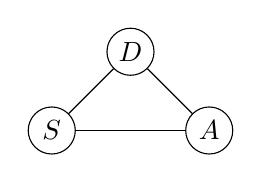
\begin{tikzpicture}
            \tikzstyle{vertex}=[circle,fill=none,draw=black,minimum size=17pt,inner sep=0pt]
\node[vertex] (S) at (0,0) {$S$};
\node[vertex] (A) at (2,0) {$A$};
\node[vertex] (D) at (1,1) {$D$};
\path (S) edge (D);
\path (D) edge (A);
\path (S) edge (A);
            \end{tikzpicture}
        \caption{$\model \in \modelsunconfedge$}
        \label{fig:no-cf-edge}
\end{subfigure}
     \begin{subfigure}{0.32\linewidth}
     \centering
            \begin{tikzpicture}
            \tikzstyle{vertex}=[circle,fill=none,draw=black,minimum size=17pt,inner sep=0pt]
\node[vertex] (S) at (0,0) {$S$};
\node[vertex] (A) at (2,0) {$A$};
\node[vertex] (D) at (1,1) {$D$};
%\node[vertex] (S') at (1,-0.5) {$S'$};
\path (S) edge (D);
\path (D) edge (A);
\path[bidirected] (D) edge[bend left=60] (A);
\path (S) edge (A);
%\path (S) edge (S'); 
% \path (S) edge node[near start, below] {=} (S');
% \draw[->, line width=0.3mm]  (S)--(D);
% \draw[->, line width=0.3mm]  (D)--(A);
% \draw[->, line width=0.3mm]  (S)--(A);
% \draw[<->, line width=0.3mm]  (D)--(A);
            \end{tikzpicture}
        \caption{$\model \in \modelsedgerelax$} 
        \label{fig:cf-edge}
        \end{subfigure}
         \begin{subfigure}{0.32\linewidth}
     \centering
            \begin{tikzpicture}
            \tikzstyle{vertex}=[circle,fill=none,draw=black,minimum size=17pt,inner sep=0pt]
\node[vertex] (S) at (0,0) {$S$};
\node[vertex] (A) at (2,0) {$A$};
\node[vertex] (D) at (1,1) {$D$};
%\node[vertex] (S') at (1,-0.5) {$S'$};
\path (S) edge (D);
\path (D) edge (A);
\path[bidirected] (D) edge[bend left=60] (A);
%\path (S) edge (A);
%\path (S) edge (S'); 
% \path (S) edge node[near start, below] {=} (S');
% \draw[->, line width=0.3mm]  (S)--(D);
% \draw[->, line width=0.3mm]  (D)--(A);
% \draw[->, line width=0.3mm]  (S)--(A);
% \draw[<->, line width=0.3mm]  (D)--(A);
            \end{tikzpicture}
        \caption{$\model \in \nullgraph$ and $\model \in \modeliv$} 
        \label{fig:cf-edge-iv}
        \end{subfigure}
        \caption{Causal graphs, $\cg{\model}$, assumed in various model classes.}
\end{figure*}

% \begin{figure}
%      \centering
%             \begin{tikzpicture}
%             \tikzstyle{vertex}=[circle,fill=none,draw=black,minimum size=17pt,inner sep=0pt]
% \node[vertex] (Z) at (0,0) {$Z$};
% \node[vertex] (Y) at (3,0) {$Y$};
% \node[vertex] (X) at (1.5,0) {$X$};
% %\node[vertex] (S') at (1,-0.5) {$S'$};
% \path (Z) edge (X);
% \path (X) edge (Y);
% \path[bidirected] (X) edge[bend left=60] (Y);
% %\path[red] (S') edge (A);
% %\path (S) edge (S'); 
%  %\path (S) edge node[near start, below] {=} (S');
% % \draw[->, line width=0.3mm]  (S)--(D);
% % \draw[->, line width=0.3mm]  (D)--(A);
% % \draw[->, line width=0.3mm]  (S)--(A);
% % \draw[<->, line width=0.3mm]  (D)--(A);
%             \end{tikzpicture}
%         \caption{Causal graph of $M \in \modeliv$} 
%         \label{fig:iv}
%         \end{figure}
\begin{abstract}

To develop generalizable models in multi-agent reinforcement learning, recent approaches have been devoted to discovering task-independent skills for each agent, which generalize across tasks and facilitate agents' cooperation. However, particularly in partially observed settings, such approaches struggle with sample efficiency and generalization capabilities due to two primary challenges: (a) How to incorporate global states into coordinating the skills of different agents? (b) How to learn generalizable and consistent skill semantics when each agent only receives partial observations? To address these challenges, we propose a framework called \textbf{M}asked \textbf{A}utoencoders for \textbf{M}ulti-\textbf{A}gent \textbf{R}einforcement \textbf{L}earning (MA2RL), which encourages agents to infer unobserved entities by reconstructing entity-states from the entity perspective. The entity perspective helps MA2RL generalize to diverse tasks with varying agent numbers and action spaces. Specifically, we treat local entity-observations as masked contexts of the global entity-states, and MA2RL can infer the latent representation of dynamically masked entities, facilitating the assignment of task-independent skills and the learning of skill semantics. Extensive experiments demonstrate that MA2RL achieves significant improvements relative to state-of-the-art approaches, demonstrating extraordinary performance, remarkable zero-shot generalization capabilities and advantageous transferability.

 % Additional rewards transform the original MTRL problem into a multi-objective MTRL problem, and the coupling relationship between the outputs of SP and ACP further complicates the optimization process. To solve this challenge, TSAC assigns a virtual expected budget to convert the multi-objective MTRL into a constrained single-objective formulation and then employs the Lagrangian method to transform a constrained single-objective optimization into an unconstrained one. The multiplier in the Lagrangian method automatically adjusts the weights during the training process, promoting cooperation between SP and ACP.
\end{abstract}
\begin{IEEEImpStatement}
The Current policies trained by Multi-Agent Reinforcement Learning (MARL) predominantly rely on meticulously designed structured environments, which considerably constrain the agents' generalization capabilities across multitasking and cross-task skill reuse. In this paper, we design a novel masked autoencoders for MARL to coordinate the skills of different agents and learn generalizable and consistent skill semantics when each agent only receives partial observations. Experimental results demonstrate that our proposed MA2RL framework significantly enhances both the asymptotic performance and generalization capabilities of the generalizable models. Specifically, MA2RL introduces masked autoencoders tailored for MARL, aimed at enhancing generalizable models. The framework holds promise for inspiring further explorations into the generalization of multi-agent reinforcement learning.
\end{IEEEImpStatement}


% Note that keywords are not normally used for peerreview papers.
\begin{IEEEkeywords}
Multi-Agent reinforcement learning, generalization, self-supervised learning.
\end{IEEEkeywords}


\IEEEpeerreviewmaketitle
% 
% 
The widespread integration of communication networks and smart devices in modern control systems has increased the vulnerability of industrial systems to online cyber-attacks, e.g., Industroyer, Blackenergy, etc \citep{osti_1505628}.
% Modern control systems have seen a large push to include communication networks and smart devices to increase performance, made possible by improvements in communication device cost and energy consumption. This trend has been coupled with the usage of open-standard communication protocols among industrial control systems, making them vulnerable to online cyber-attacks such as Industroyer, Blackenergy, etc \citep{osti_1505628}. 
To counter this, methods have been developed to improve security by achieving attack detection, mitigation, and monitoring, among others \citep{sandberg2022secure}. This paper focuses on active attack diagnosis to mitigate stealthy attacks. 
%
%\subsection{Literature review}

Active diagnosis techniques rely on the inclusion of additional moduli to control systems
% inclusion within the control system of additional moduli 
to alter the behavior of the system compared to information known by the attacker. 
For instance, the concept of additive watermarking was introduced in \cite{mo2015physical}, where noise signals of known mean and variance are added at the plant and compensated for it at the controller. 
This compensation, however, is not exact, causing some performance degradation. Thus, trade-offs between performance and detectability  are necessary \citep{zhu2023detection}.
% A later work \citep{zhu2023detection} designs the watermark signal by trading performance for detection. Thus, although additive watermarking serves as a good detection scheme, they endure performance losses even in the nominal case. 

In encrypted control \citep{darup2021encrypted}, the sensor data is encrypted, sent to the controller, and then operated on directly. Encrypted input signals are sent back to the plant for decryption. Although encryption is widespread in IT security, in control systems it presents some concerns, such as the introduction of time delays \citep{stabile2024verifiable}, while it may present inherent weaknesses \citep{alisic2023model}.
% they are not preferred as they introduce time delays \citep{stabile2024verifiable} which can cause instability, and some encryption schemes can be very weak  \citep{alisic2023model}. 

In moving target defense \citep{griffioen2020moving}, the plant is augmented with fictitious dynamics, known to the controller. The plant output is transmitted to the controller along with the fictitious states over a network under attack. 
The additional measurements then aide in the detection of attacks. 
This comes at the cost of higher communication bandwidth needs, which increases rapidly with the dimension of the augmented systems.
% Since the dynamics of the fictitious dynamics are exactly known to the controller, the attack is detected easily. However, when the scale of the system increases, the communication bandwidth used by moving the target defense approach increases rapidly. 

Other recently proposed works include two-way coding \citep{fang2019two}, a weak encryuption technique, and dynamic masking \citep{abdalmoaty2023privacy}, which enhances privacy as well as security, have been shown to be effective against zero-dynamics attacks.
% Two-way coding \citep{fang2019two} and dynamic masking \citep{abdalmoaty2023privacy} are other recently proposed approaches. Two-way coding is another form of weak encryption technique whilst dynamic masking proposes an architecture that enhances both privacy and security. These schemes are shown to be effective against zero dynamics attacks but remain to be studied for other classes of attacks. 
% Recent extensions include \citep{mukherjee2021secure,ramos2024privacy}.
% Some other works which are related are \citep{mukherjee2021secure}, an extension of \cite{fang2019two}. The work \citep{ramos2024privacy} is an extension of moving target defense for multi-agent systems. 
Furthermore, filtering techniques for attack detection are proposed by \cite{murguia2020security,hashemi2022codesign,escudero2023safety}, while not focusing on stealthy attacks.
% The works \citep{murguia2020security,hashemi2022codesign,escudero2023safety} develop filtering techniques to guarantee safety, without being focused on stealthy covert attacks.

Multiplicative watermarking (mWM) has been proposed by the authors as a diagnosis technique \citep{ferrari2020switching}. mWM consists of a pair of filters on each communication channel between the plant and its controller; the scheme is affine to weak encryption, whereby ``encoding'' and ``decoding'' are done by changing signals' dynamic characteristics through inverse pairs of filters. This enables original signals to be recovered exactly, and thus does not lead to performance degradation.
% A multiplicative watermark is an affine to a weak encryption technique, through which the signal is ``encoded'' by a filter, changing its dynamic behavior. The use of inverse pairs means that the original signal can be recovered, through ``decoding'' via an inverse filter. As such, differently to techniques based on additive watermarking, no performance is lost due to the injection of noise, and there are no bandwidth limitations.

%\subsection{Contributions}
One of the critical features of multiplicative watermarking is that to detect stealthy attacks, the mWM filter parameters must be switched over time. In this paper, an algorithm to optimally design the mWM parameters after a switching event is presented, enhancing detection performance, without changing the switching time.
% This is done without changing the switching time, which is taken as given.

\textcolor{black}{
To formalize the filter design problem, we suppose the defender is interested in optimal performance against adversaries injecting covert attacks with matched system parameters \citep{smith2015covert}, including the mWM parameters prior to the switch. This scenario represents a worst case where malicious agents can take full control of the system while remaining undetected.
Thus, the attack strategy is explicitly included within the formulation of the closed-loop system, and the mWM filters are chosen by solving an optimization problem minimizing the attack-energy-constrained output-to-output gain (AEC-OOG) \citep{anand2023risk}, a variation of the output-to-output gain proposed in  \cite{teixeira2015strategic}.
}
The main contributions of this paper are:
% We consider an adversary injecting a covert attack with matched system parameters \citep{smith2015covert}, i.e., an attacker with full knowledge of the control system parameters, including those of the mWM filters before the switch. This scenario is taken as a worst case, as it has been shown that this class of attacks can be made stealthy. To quantitatively define a cost, the output-to-output gain (OOG) \citep{teixeira2015strategic} is leveraged,
% a metric introduced to evaluate the impact of an additive attack in a control system. %Specifically, OOG evaluates the worst-case performance loss that an attacker injecting an undetectable attack can obtain. 
% Here, the maximum performance loss caused by a stealthy adversary with limited energy is taken, the attack-energy-constrained OOG (AEC-OOG) \citep{anand2023risk}. The main contributions of this paper are:
\begin{enumerate}
%[label=\alph*.]
\item The problem of optimally designing the switching mWM filters is formulated as an optimization problem, with the AEC-OOG is taken as the objective;%where the AEC-OOG is taken as the impact metric; 
\item The worst-case scenario of a covert attack with exact knowledge of plant and mWM filter parameters is embedded within the design problem;
% The optimization problem is defined to incorporate the worst-case scenario of a covert attack with exact knowledge of plant and mWM filter parameters;
\item The feasibility of the optimization problem is shown to be dependent only on stability conditions; 
\item A solution scheme is proposed to promote randomization of the mWM filter parameters such that an eavesdropping adversary cannot remain stealthy.
\end{enumerate} 

This builds on the results of \cite{ferrari2020switching}, where the focus was on the design of the switching protocols, rather than the parameters themselves.
Compared to previous work \citep{gallo2021design}, this paper introduces an optimization problem which is always feasible (thanks to the use of AEC-OOG in the objective), while also considering a more sophisticated class of covert attacks, where the presence of watermark is known to the adversary. 
Moreover, this paper poses a different objective than \citep{zhang2023hybrid}; indeed, while \citep{zhang2023hybrid} provided a design strategy to ensure certain privacy properties, in this paper we address the problem of optimal parameter design following a switching event.


%\subsection{Organization}
The rest of the paper is organized as follows. 
After formulating the problem in Section~\ref{sec:PF}, we propose our design algorithm in Section~\ref{sec:main}, and analyze its properties. It is then evaluated through a numerical example in Section~\ref{sec:NE}, and concluding remarks are given Section~\ref{sec:Con}.
% We provide the problem background in Section~\ref{sec:PF}. We formulate the design problem in Section~\ref{sec:main}, together with an analysis of its properties. The proposed algorithm is evaluated through a numerical example in Section \ref{sec:NE}. Concluding remarks are offered in Section \ref{sec:Con}.
\section{Related works}
Implicit Neural Representations are designed to learn continuous representations of target functions by taking advantages of the approximation power of neural networks.
%
Their inherent continuous property can beneficial in many cases like video compression~\citep{chen2021nerv,strumpler2022implicit}, 3D modeling~\citep{park2019deepsdf,atzmon2020sal,9010266,gropp2020implicit,sitzmann2019scene} and volume rendering~\citep{pumarola2021d, barron2021mip,martin2021nerf,barron2023zip}.
%
However, simply employing MLPs may result in spectral bias, where oversmoothed outputs are generated due to the inherent tendency of MLPs to prioritize learning low-frequency components first. Consequently, many studies have focused on these drawbacks and explored various methods to address this issue.
%
The most straightforward way to address this issue is by projecting the coordinates into the higher dimension~\citep{tancik2020fourier, wang2021spline}.
%
However, these methods can lead to noisy outputs if there is a mismatch in the embeddings variance.
%
To address this, \citet{landgraf2022pins} propose dividing the Random Fourier Features into multiple levels of detail, allowing the MLPs to disregard unnecessary high-frequency components. Another type of approach to mitigating the spectral bias introduced by the ReLU activation function, as proposed by \citet{sitzmann2020implicit}, \citet{ramasinghe2022beyond}, \citet{saragadam2023wire}, and \citet{shenouda2024relus}, is to modify the activation function itself by using alternatives such as the Sine function, Wavelets, or a combination of ReLU with other functions. There are also efforts to modify network structures to mitigate spectral bias~\citep{mujkanovic2024neural}. 
%
\citet{lindell2022bacon} introduce a network design that treats MLPs as filters applied to the input of the next layer, known as Multiplicative Filter Networks (MFNs). 
%
Additionally, based on the discrete nature of signals like images and videos, grid-based approaches (e.g., Grid Tangent Kernel~\citep{zhao2024grounding}, DINER~\citep{xie2023diner}, and Fourier Filter Bank~\citep{wu2023neural}) have been proposed to address spectral bias, as the grid property allows for sharp changes in features, which facilitates learning fine details.
Even though, there are some prior works trying to solve the inherent problems of Fourier features embeddings ~\citep{landgraf2022pins, yuce2022structured, hertz2021sape, saratchandran2024sampling}, limited research has addressed both the underlying causes of high-frequency noise and provides a non-heuristic solution even if these embeddings are widely employed into many downstream tasks.

\begin{figure*}
	\centering
	\includegraphics[width = \linewidth]{figure/AgentArena.pdf}
	\caption{\textbf{Stock Trading Workflow in \textit{Agent Trading Arena}.} 
	\textbf{Top:} Workflow of a trading day, including preparation, trading, and post-trading reflection. Agents discuss insights in the chat pool, analyze market trends, execute trades, and refine strategies based on performance.  
	\textbf{Bottom:} Example of agents' interactions in the chat pool and dynamic strategy updates.}
	\label{fig:AgentArena}
	\vspace{-3pt}
\end{figure*}

\section{Proposed Method}

% 核心部分visual representation,

To mitigate the influence of human prior knowledge and memory, we designed a closed-loop economic system~\citep{guo2024economics} called the \textit{Agent Trading Arena}, a zero-sum game simulating complex, quantitative real-world scenarios. The simulation workflow is illustrated in \autoref{fig:AgentArena} and further detailed in \autoref{appendix_arena}. In the \textit{Agent Trading Arena}, agents can invest in assets, earn dividends from holding assets, and pay daily expenses using virtual currency. The agent with the highest total return wins the game.

\subsection{Agent Trading Arena}

\paragraph{Structure of Agent Trading Arena.} 

To eliminate external knowledge biases, asset prices are determined by a bid-ask system, reflecting the prices at which buyers and sellers are willing to transact. The system evolves solely based on agents' actions and interactions, without external influences. This design ensures that the outcomes of agents' actions are not immediately apparent but unfold gradually, influenced by other agents' decisions.

To encourage active participation, a dividend mechanism is introduced. There are two primary sources of income in this system: capital gains from asset price differentials and dividends from holding assets. Dividends for each asset are distributed according to a predefined ratio, serving as an implicit anchor for asset prices. Agents holding more low-cost assets receive higher dividends. To prevent passive asset holding until the end of the game, agents must pay a daily capital cost proportional to their total wealth. These expenses are offset by asset dividends, and only agents with sufficient low-cost assets can cover costs. Under the pressure of significant daily expenses, agents must act swiftly and strategically, triggering frequent trades and price fluctuations to stimulate market activity. This dynamic mechanism ensures fairness in the zero-sum game while preventing agents from relying on fixed strategies to find optimal solutions.

\vspace{-3pt}

\paragraph{Agents Learn and Compete in Arena.}

The zero-sum game structure is crucial to eliminating the possibility of a universally optimal strategy. In fixed scenarios with a static optimal solution, agents could rely on predefined rules or memory-based approaches, bypassing adaptive decision-making. The zero-sum game ensures that there is no universally correct solution, with outcomes evolving dynamically based on agent interactions and competition. This design forces agents to continually adapt, learn from feedback, and develop context-dependent strategies, promoting deeper environmental exploration and preventing reliance on static or memory-driven solutions.

In the \textit{Agent Trading Arena}, agents are unaware of implicit rules, except for the objective to maximize their virtual wealth throughout the simulation. To win this zero-sum game, agents must effectively learn from experience, decipher hidden game rules, and develop strategies to counter competitors. This requires the ability to comprehend numerical feedback, formulate enduring strategies, and make informed decisions. Unlike other mathematical reasoning problems, the results of their actions unfold gradually and dynamically. Moreover, agents are easily misled by erroneous information from competitors, hindering their ability to discern strategic cues from competitors' textual data. Importantly, agents remain unaware of these implicit rules, so applying real-world knowledge does not benefit their performance. Therefore, agents must rely on experiential learning to decipher the hidden game rules and ultimately achieve victory.

\subsection{Types of Numerical Data Input}

\paragraph{Limitations of Textual Numerical Data.}

In the \textit{Agent Trading Arena}, the generated stock data is stored in numerical format. When used directly as input to an LLM, the models often struggle to interpret numerical data accurately or make sound decisions. To mitigate this, we convert the data into textual formats~\citep{numerical_text, long_text}, enhancing semantic features and clarifying output requirements to improve the models' understanding. During interactions, the LLMs process stock prices, trading volumes, and market indices presented as textual numerical data.

\begin{figure*}
	\centering
	\includegraphics[width = \linewidth]{figure/v_t.pdf}
	\caption{\textbf{Textual and Visual Representations of Corresponding Inputs and Outputs.} The left images display the agent’s Buy and Sell trading records, daily trade prices, and K-line charts for three stocks. The output from visual inputs (bottom right) captures overall stock trends and long-term behavior, while the output from textual inputs (top right) focuses on specific current prices.}
	\label{textual_visualized}
	\vspace{-3pt}
\end{figure*}

However, this textual approach reveals significant limitations. While the data is presented clearly, LLMs tend to focus excessively on specific values rather than identifying long-term trends or global patterns. They also struggle with understanding correlative relations and percentage changes, limiting their ability to assess differences and identify connections between data points. When analyzing time-series data with complex patterns, LLMs often fixate on individual data points, overlooking overarching relations. This issue is evident in the analysis output in the top-right corner of \autoref{textual_visualized}, where LLMs' focus on individual values impedes their ability to generalize, reducing their capacity to extract meaningful global insights.

Additionally, LLMs often overemphasize recent data while undervaluing historical information, even when prompted to consider its importance. This prevents them from effectively integrating past data and recognizing long-term patterns, complicating their understanding of numerical relations and trends. These challenges highlight the need for improved mechanisms to process numerical relations, identify global trends, and derive deeper insights from textual numerical data.

\vspace{-3pt}

\paragraph{Potential of Visual Numerical Data.}

Since textual numerical data often leads LLMs to focus on local details while neglecting broader relations, we investigated whether visual representations, such as scatter plots, line charts, and bar charts, could help LLMs better understand overall trends, similar to human reasoning. Thus, we transition from textual numerical data inputs to visualized formats ~\citep{storyllava}. As demonstrated in the bottom-right corner of \autoref{textual_visualized}, visual representations enable LLMs to more effectively grasp global trends, patterns, and relations that are often difficult to discern from textual numerical data alone.

These findings highlight the advantages of structured, visual numerical data, indicating that this format allows LLMs to more intuitively and comprehensively understand complex data, better capturing overall fluctuations, whereas text tends to focus on local details. By combining visualization and textual representations, LLMs not only overcome the challenges of relations in time-series data but also demonstrate better performance in identifying long-term trends and global patterns, while still attending to local details.

\subsection{Reflection Module}

We propose a strategy distillation method, illustrated in \autoref{fig:reflection}, that delivers real-time feedback to LLMs by analyzing both descriptive textual and visual numerical data. This enables the generation of new strategies and optimization of action plans. The approach allows agents to evaluate their results, refine strategies, and adapt continuously based on feedback. The process begins with assessing the day’s trajectory memory and associated strategies using an evaluation function. The strategic generation process leverages contrastive analysis of peak and nadir performers from the evaluation phase, creating bidirectional learning signals that inform subsequent iterations. This iterative cycle ensures continuous strategy evolution, fostering sustained improvement in decision-making.

\begin{figure}[t]
	\centering
	\includegraphics[width = \linewidth]{figure/reflection.pdf}
	\caption{\textbf{Design of the Reflection Module.} The process evaluates daily trajectory memory and strategies (top right), then generates new strategies (center) based on evaluation, environmental feedback (bottom right), and feedback from the 5 top- and bottom-performing strategies. Stock visualization (bottom left) enhances reflection, driving continuous improvement.}
	%The process evaluates daily trajectory memory and strategies, generating new strategies based on positive and negative feedback from the top- and bottom-performing strategies. Stock visualizations (bottom left) further enhance the reflection process, reinforcing continuous strategy refinement.}
	\label{fig:reflection}
	\vspace{-3pt}
\end{figure}

% We propose a strategy distillation method, illustrated in \autoref{fig:reflection}, that provides real-time feedback to LLMs by analyzing both descriptive textual and visualized numerical data. This enables the generation of new strategies and the optimization of action plans. The approach allows agents to assess their results, refine strategies, and continuously adapt based on feedback. The process begins by evaluating the day's trajectory memory and associated strategies using an evaluation function. From this assessment, new strategies are generated by selecting the top-performing and lowest-performing strategies, offering both positive and negative feedback. This iterative cycle ensures continuous strategy evolution, driving sustained improvement in decision-making.

The reflection module plays a crucial role in refining strategies by offering real-time feedback. It analyzes both descriptive textual and visual numerical data to generate new strategies and optimize action plans. Within the \textit{Agent Trading Arena}, the reflection module is triggered regularly to consolidate daily trading records and evaluate the effectiveness of strategies, refining both successful and unsuccessful experiences to guide future decisions. Ineffective strategies are stored in a strategy library for future reference, allowing agents to review and learn from past experiences. Further details can be found in \autoref{appendix_arena}.


\newpage
\section{Experiment}\label{sec-experiment}
\subsection{Experimental Setup}
We briefly introduce experimental settings to verify our proposed MoR, including Datasets \& Baselines, Implementation Details, and Evaluation Metrics. More details are in Appendix~\ref{app-expr-setting}.

\textbf{Datasets \& Baselines:} We use three TG-KBs from STaRK~\cite{wu2024stark} covering three knowledge domains, including E-commerce Products (Amazon), Academic Papers (MAG), and Biomedicine (Prime). We compare our MoR with baselines established by~\citet{wu2024stark} and categorize them into textual/structural/hybrid-based ones. More recent state-of-the-art hybird retrieval approaches fro TG-KBs such as KAR~\cite{xia2024knowledge} and MFAR$^{*}$~\cite{li2024multi} are also compared.


\textbf{Implementation Details:} 
To enhance the planning capability of our planning module, we fine-tune the Llama 3.2 (3B) on 1000 sampled queries with their corresponding ground-truth planning graphs, serving as the textual graph generator. In the absence of ground-truths, we synthesize them using LLMs. For the Prime dataset, we empirically find that directly prompting LLMs can hardly generate accurate planning graphs due to the lack of biomedical domain knowledge~\cite{Shen2024TagLLMRG}. Therefore, we adopt an alternative approach. First, we instruct LLMs to extract triplets from each query and then construct the planning graphs by merging triplets with shared entities. 
During mixed traversal, textual matching can be implemented using any lexical or semantic methods. For this study, we employ BM25 for Amazon and MAG and fine-tune a contriever to complement the biomedical knowledge for Prime.
To initialize the structural traversal, we employ textual matching to locate the top 5 nodes that are most relevant to the query as seeds. Additionally, at each layer, we incorporate the top 10 nodes retrieved via textual matching and append them to the current candidate set for the next round of traversal. Notably, due to the uncertainty of LLMs, the generated planning graphs can be invalid. In this case, we will directly conduct textual matching to retrieve candidates. For our ablations without reranker, we employ Ada-002~\cite{wu2024stark} with cosine similarity as the scorer to rank candidates for evaluating performance.

\textbf{Evaluation Metrics:}
We follow~\citet{wu2024stark} for evaluation by reporting Hit@1 (H@1), Hit@5 (H@5), Recall@20 (R@20), and mean reciprocal rank MRR to evaluate in the full spectrum. 


 

\newpage
\subsection{Overall Retrieval Performance}
We compare MoR with other baselines on three TG-KBs in Table~\ref{tab-merged}. Generally, hybrid methods, AvaTAR, KAR, MFAR$^{*}$, and our MoR, achieve better performance than purely textual or structural methods owing to their ability to integrate both structural and textual knowledge. 
Among all baselines, our proposed MoR achieves the overall best performance with a substantial margin on average, with the first ranking on MAG and the second ranking on Amazon/Prime datasets. This demonstrates the effectiveness of our proposed mixture of structural and textual knowledge retrieval. 
Textual retrieval performs better on Amazon than on MAG, suggesting that Amazon queries rely more on textual knowledge. In contrast, its weaker performance on MAG is due to MAG's lower textual richness and stronger structural signals. This disparity aligns with the distribution analysis presented by~\citet{wu2024stark} and supports our hypothesis that queries in different TG-KB datasets require varying desires for textual and structural knowledge. Meanwhile, structural retrieval methods such as conventional knowledge graph-based ones perform poorly because they are designed for graphs with minimal textual information compared to TG-KBs.
Different from Amazon and MAG, all existing methods without supervised tuning (e.g., Ada-002) exhibit significantly lower performance on Prime. This is due to the extreme domain expertise required in biology, where word-count-based, pre-trained textual similarity-based, and even more powerful LLMs are all poorly applicable here. Through fine-tuning, MFAR$^{*}$ and our proposed MoR generally achieve better performance, demonstrating the necessity of domain-specific knowledge for answering queries in knowledge-intensive domains. 




\newpage
\subsection{Ablation Study}
After verifying the superiority of MoR, we conduct ablation studies to assess its different components, including module and feature ablation.

\subsubsection{Module Ablation}


To assess the contribution of each module in MoR, namely, Text Matching-based Retrieval, Neighborhood-Fetching-based Structural Retrieval, and Reranker, we conduct a series of ablation experiments. First, we remove the Reranker, resulting in the variant MoR$_{\text{w/o R}}$. On top of that, we further separately eliminate Text Retrieval and Structural Retrieval, yielding MoR$_{\text{w/o RT}}$ and MoR$_{\text{w/o RS}}$, respectively.
As shown in Table~\ref{tab-merged}, the complete MoR framework consistently achieves the highest performance across all datasets, demonstrating the synergistic effect of the Textual Retriever, Structural Retriever, and Reranker.
After removing Reranker, MoR$_{\text{w/o R}}$ exhibits a consistent performance drop across all datasets and evaluation metrics. This underscores the importance of the Reranker in refining retrieval by filtering noisy candidates from the intermediate reasoning stage. 
Eliminating Text Retrieval, i.e., MoR$_{\text{w/o RT}}$, leads to a notable performance drop on Amazon but an unexpected improvement on MAG. This suggests that while textual knowledge benefits Amazon, it introduces misleading hard negatives that compromise the ranking method (e.g., Ada-002) for MAG. Conversely, removing Structural Retrieval, MoR$_{\text{w/o RS}}$, results in a slight performance decrease further on MAG, reinforcing the importance of structural knowledge in MAG-related queries.
%
These results underscore the Reranker's crucial role in adaptively harmonizing, balancing, and selecting knowledge from both structural and textual retrieval experts.






\begin{table}[t!]
\small
\setlength\tabcolsep{4.5pt}
\centering
\begin{tabular}{l|ccc|cccc}
\toprule
\textbf{Dataset} &\textbf{TF} & \textbf{SF} & \textbf{TI} & \textbf{H@1} & \textbf{H@5} & \textbf{R@20} & \textbf{MRR} \\ \midrule
\multirow{7}{*}{\textbf{MAG}} 
& \cmark & \xmark & \xmark & 48.96 & 73.02 & 72.44 & 59.79 \\
&      \xmark            & \cmark       &         \xmark         & 18.79 & 41.91 & 52.85 & 29.84 \\
&        \xmark          &         \xmark         & \cmark       & 18.16 & 41.53 & 52.78 & 29.31 \\
\cline{2-8}
& \cmark       & \cmark       &    \xmark              & 58.04 & 77.14 & 74.42 & 66.75 \\
& \cmark       &        \xmark          & \cmark       & \underline{58.16} & \underline{77.59} & \underline{74.96} & \underline{66.85} \\
&          \xmark        & \cmark       & \cmark       & 17.93 & 38.01 & 46.79 & 27.48 \\
\cline{2-8}
& \cmark       & \cmark       & \cmark       & \textbf{58.19} & \textbf{78.34} & \textbf{75.01} & \textbf{67.14} \\ \midrule
\multirow{7}{*}{\textbf{Amazon}}    
& \cmark       &      \xmark            &       \xmark           & \underline{51.21} & \underline{74.05} & \underline{59.79} & \underline{61.27} \\
&        \xmark          & \cmark       &      \xmark            & 8.09  & 24.48 & 25.62 & 16.94 \\
&         \xmark         &      \xmark            & \cmark       & 5.84  & 16.62 & 12.94 & 11.57 \\
\cline{2-8}
& \cmark       & \cmark       &      \xmark            & 50.91 & 73.38 & 59.58 & 61.15 \\
& \cmark       &         \xmark         & \cmark       & 51.09 & 73.56 & 59.61 & 61.14 \\
&            \xmark      & \cmark       & \cmark       & 8.09  & 24.48 & 25.62 & 16.94 \\
\cline{2-8}
& \cmark       & \cmark       & \cmark       & \textbf{52.19} & \textbf{74.65} & \textbf{59.92} & \textbf{62.24} \\ \bottomrule
\end{tabular}
\caption{Ablation study investigating the importance of three features, Textual Fingerprint (\textbf{TF}), Structural Fingerprint (\textbf{SF}), and Traversal Identifier (\textbf{TI}), of the traversal trajectories used in our Structure-aware Reranker.}
\label{tab-feature-ablation}
\vspace{-2ex}
\end{table}



\subsubsection{Feature Ablation}
The above ablation study highlights the crucial role of Structure-aware Reranker in adaptively integrating structural and textual knowledge. To further analyze the contributions of its three key features, \textbf{Textual Fingerprint (TF)}, \textbf{Structural Fingerprint (SF)}, and \textbf{Traversal Identifier (TI)} defined in Section~\ref{sec-organizing}, we conduct a feature ablation analysis and report retrieval performance across different feature configurations in Table~\ref{tab-feature-ablation}.
%Overall and individual performance
Overall, using three features together yields the best performance on both MAG and Amazon, highlighting their synergistic effect. Individually, TF contributes the most and outperforms SF and TI on both datasets. 
The reason is that based on the definition in Section~\ref{sec-organizing}, TF directly captures the relevance between the query and the retrieved nodes along the trajectory, whereas SF and TI primarily characterize the structural patterns and retrieval types, serving more as complementary factors. Therefore, equipping TF with these complementary factors (i.e., SF or TI) yields around 10\% additional gains on MAG. This is because SF and TI help the reranker selectively emphasize the relevance scores given by TF for certain nodes along the path. However, this boost is not observed on Amazon. We hypothesize that the textual knowledge needed there is predominantly derived from the final node on each path, making the structural cues provided by SF and TI less beneficial and even prone to overfitting. A deeper analysis to further justify this hypothesis is in Section~\ref{sec-further}. Overall, these findings underscore the varying importance of structural features in ranking across datasets.



\begin{table}[t!]
\small
\setlength\tabcolsep{4pt}
\centering
\begin{tabular}{l|ccc|ccc}
\toprule
\multirow{2}{*}{\textbf{Feature}} & \multicolumn{3}{c|}{\textbf{MAG}} & \multicolumn{3}{c}{\textbf{Amazon}} \\

 & H@1 & R@20 & MRR & H@1 & R@20 & MRR \\
\midrule
Last Node & 49.91 & 73.49 & 59.92 & 50.36 & 59.62 & 61.05   \\
Full Path & \textbf{58.19} & \textbf{75.01} & \textbf{67.14} & \textbf{52.19} & \textbf{59.92} & \textbf{62.24}   \\
\bottomrule
\end{tabular}
\caption{Comparing reranking performance using last node in the retrieved trajectory and the whole trajectory.}
\label{tab-Reranker-ablation}
\vspace{-2ex}
\end{table}

\begin{figure}[t!]
    \centering
    \includegraphics[width=0.49\textwidth, height = 0.22\textwidth]{figures/query-pattern-20250215.png}
    \vspace{-4.5ex}
    \caption{Imbalance number of queries and performance of different retrievers across different logical structures.}
    \label{fig-analysis}
    \vspace{-3ex}
\end{figure}





\subsection{Further Analysis}\label{sec-further}
This section understands MoR’s behavior by examining three questions, each of which enriches our insight into MoR’s functionality and offers novel perspectives inspiring future query retrieval research.

\textbf{Do structure signals affect reranking?}
To assess the impact of trajectory information on the Reranker's decision-making, we introduce a node-based Reranker that constructs trajectory features using only TF/SF/TI of the last node. In Table~\ref{tab-Reranker-ablation}, the path-based Reranker outperforms the node-based variant, especially on MAG. This highlights the critical role of trajectory features/structural knowledge in reranking. The minor performance boost on Amazon after switching to the full path trajectory indicates its textual knowledge preference over the last node rather than the whole trajectory.


\textbf{How does MoR perform on different logical structures?}
Figure~\ref{fig-analysis} shows the average performance of MoR on each query group categorized by their logical structures, where "Others" refer to queries with undefined logical structures in~\citet{wu2024stark} MoR consistently outperforms structural and textual retrievers across different logical structures. Among all queries, MoR performs the worst on "P → P" queries due to the ambiguity, although well-known, uniquely caused by repeated product entities from multi-step traversal.
The average-performing ``Others" group underscores the utility of diverse planning strategies for the same query.
Lastly, the skewed query distribution and retrieval performance across planning patterns reflect the varying nature of real-world planning needs. We hope these insights inspire research on data-centric reasoning designs and error control of planning.


\begin{figure}[t!]
    \centering
    \includegraphics[width=0.5\textwidth]{figures/heatmap-20250215.pdf}
    \vspace{-3ex}
    \caption{Saliency map visualization of query attention over three entities along the retrieved paths}
    \label{fig-map}
    \vspace{-2ex}
\end{figure}

\textbf{Does MoR indeed adaptively leverage the trajectory knowledge?} To understand how our proposed reranker prioritizes candidates in the Top-K results, we visualize the saliency map by computing the gradient of ranking scores with respect to the textual fingerprint (TF) of three nodes along the traversed path, which quantifies their importance for answering a given query. Figure~\ref{fig-map} illustrates this by analyzing trajectories for 100 ground-truth candidates across 100 queries on the Amazon and MAG datasets. Each dimension corresponds to a traversed node, with the final one representing the candidate itself. 
While the saliency score is concentrated in the last dimension for Amazon, 
MAG exhibits a more evenly distributed saliency pattern, where multiple nodes along the path contribute significantly to ranking score computation. This suggests that structural knowledge is more critical for answering queries in MAG, aligning with the previously observed lower performance of purely textual retrieval on MAG in Table~\ref{tab-merged}. Further case studies explain why the reranker attends different nodes for different queries. In Figure~\ref{fig-map}(a), the reranker favors the last two dimensions as the rich textual restriction (i.e., "Northwest Company..." and "NFL Seattle...") aids in identifying the correct node at the corresponding reasoning step, as discussed in Section~\ref{sec-reasoning}. The correct nodes, having higher similarity scores with the query, help guide the retrieval process toward the ground truth.
Conversely, in Figure~\ref{fig-map}(b),
since the first node ("University of Lausanne") helps narrow the search space and the last node ("frameless...") further filter candidates, both nodes have high saliency scores. Overall, our findings demonstrate that the reranker dynamically adapts its reliance on structural and textual knowledge depending on the dataset and query. 

Software development is increasingly conceived as a collaboration activity between developers and AIs. Indeed, IDEs already implement features to enable interactive development, with AI suggesting implementations that are reused by developers.

Although multiple studies show this interaction can be successful, there is still limited understanding of how the models must be configured and used in the context of code generation tasks. This study addresses this gap, systematically investigating the impact of several key parameters, including the repeated submission of a prompt to accommodate for the non-deterministic nature of the models.

Our study reveals several key findings about the usage of ChatGPT. In particular, we discovered how creativity, although up to a limited extent, is useful to increase the range of methods whose code can be generated correctly. A major role is played by parameter top-p, which is commonly underrated, and instead has a major impact on the correctness of the results, with lower values producing better results. Finally, prompts should be submitted multiple times, with $5$ repetitions combined with a temperature of $1.2$ resulting in an effective configuration in our experiments.  

Future work concerns two main research directions. One is about replicating this experiment with other AI assistants, to validate our findings in multiple contexts. The second research direction concerns finding strategies to deal with the need to submit the same prompt multiple times to obtain a useful result, and thus developing approaches able to select or merge multiple responses automatically. 

\newpage

%%%%%%%%%%%%%%%%%%%%%%%%%%%%%%%%%%%%%%%%%%%%%%%%%%%%%%%%%%%%%%%%%%%%%%%%%%%%%%%%
\bibliographystyle{./IEEEtran}
\bibliography{./IEEEabrv,./IEEEexample}




\end{document}
